\documentclass{article}
%\VignetteIndexEntry{Historical Studies}

\usepackage{parskip}
\usepackage[a4paper, total={6.5in,9in}]{geometry}
\usepackage{natbib}

\usepackage{Sweave}
\begin{document}

\author{Isaac Gravestock}
\title{StudyPrior for Binary Outcomes}
\maketitle

The StudyPrior package implements a number of Bayesian priors used for clinical trials. 
This vignette shows the methods for trials with a binary outcome.

\section{StudyPrior for a Single Historical Study}

StudyPrior implements a number of methods that are suitable for creating priors for the success probability $\theta$ based on a single historical study. 
If a previous study under similar conditions had 21 successes for 37 subjects, we can use this to construct a prior using power prior (PP) methodology.
\begin{Schunk}
\begin{Sinput}
> library(StudyPrior)
> x <- 21
> n <- 37
> #Full Bayes with delta~Be(1,1)
> pp.fullbayes.11 <- binom.PP.FB.MC.BE(x = x, n = n, d.prior.a = 1, d.prior.b = 1) 
> #Full Bayes with delta~Be(.5,.5)
> pp.fullbayes.55 <- binom.PP.FB.MC.BE(x = x, n = n, d.prior.a = .5, d.prior.b = .5) 
> #Power prior with fixed delta=0.8
> pp.fix.08 <- binom.PP.FIX(x=x, n=n, d=0.8) 
\end{Sinput}
\end{Schunk}

These priors returned in the form of a density function for a single probability parameter. 

We can also fit an empirical Bayes (EB) prior based on the new study, with say 50 patients.
\begin{Schunk}
\begin{Sinput}
> n.new <- 50
> pp.eb <- binom.PP.EB(x=x, n=n, X=0:n.new, N=n.new)
\end{Sinput}
\end{Schunk}

We can plot priors. The EB prior requires the number of successes in the new trial, say 30.
\begin{Schunk}
\begin{Sinput}
> plot(pp.fullbayes.11, col="red",
+      xlim=c(0,1), ylim=c(0,6), ylab="Density", 
+      xlab=expression(paste("Success Probability",~theta)))
> curve(pp.fullbayes.55, add=TRUE, col="blue")
> curve(pp.fix.08, add=TRUE, col="green")
> curve(pp.eb(x,30), add=TRUE, col="orange")
> legend("topleft", col=c("red","blue","green", "orange"), lty=1, lwd=2,
+        legend=c("Full Bayes PP B(1,1)", "Full Bayes PP B(.5,.5)",
+                 "Fixed PP d=0.8", "Empirical Bayes PP"))
\end{Sinput}
\end{Schunk}
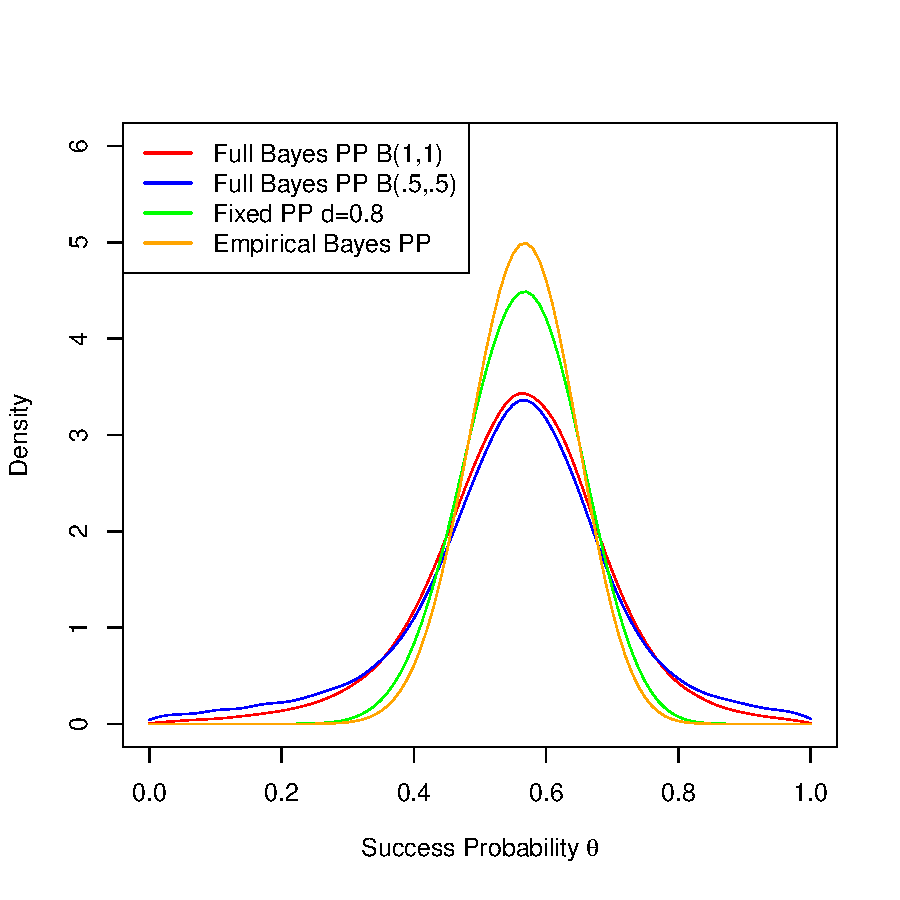
\includegraphics{Binomial-plot}
\subsection{Operating Characteristics}

Useful functions such as calc.MSE are available to calculate operating characteristics.
\begin{Schunk}
\begin{Sinput}
> MSE <- sapply(list(pp.fullbayes.11, pp.fullbayes.55, pp.fix.08, pp.eb),
+               function(PRIOR) calc.MSE(prior=PRIOR, 
+           prob.range = c(0.3,0.8), length = 11, n.binom=n.new))
> p <- seq(0.3,0.8,len=11)
> plot(p,MSE[,1],  col="red" , pch=16, type='l',
+      ylab="MSE", xlab=expression(paste("Success Probability ",theta)),
+      ylim=c(0.005,0.015))
> lines(p,MSE[,2],  col="blue", pch=16)
> lines(p,MSE[,3],  col="green", pch=16)
> lines(p,MSE[,4],  col="orange", pch=16)
> legend("top", col=c("red","blue","green", "orange"), lty=1, lwd=2,
+        legend=c("Full Bayes PP B(1,1)", "Full Bayes PP B(.5,.5)",
+                 "Fixed PP d=0.8", "Empirical Bayes PP"))
> 
\end{Sinput}
\end{Schunk}
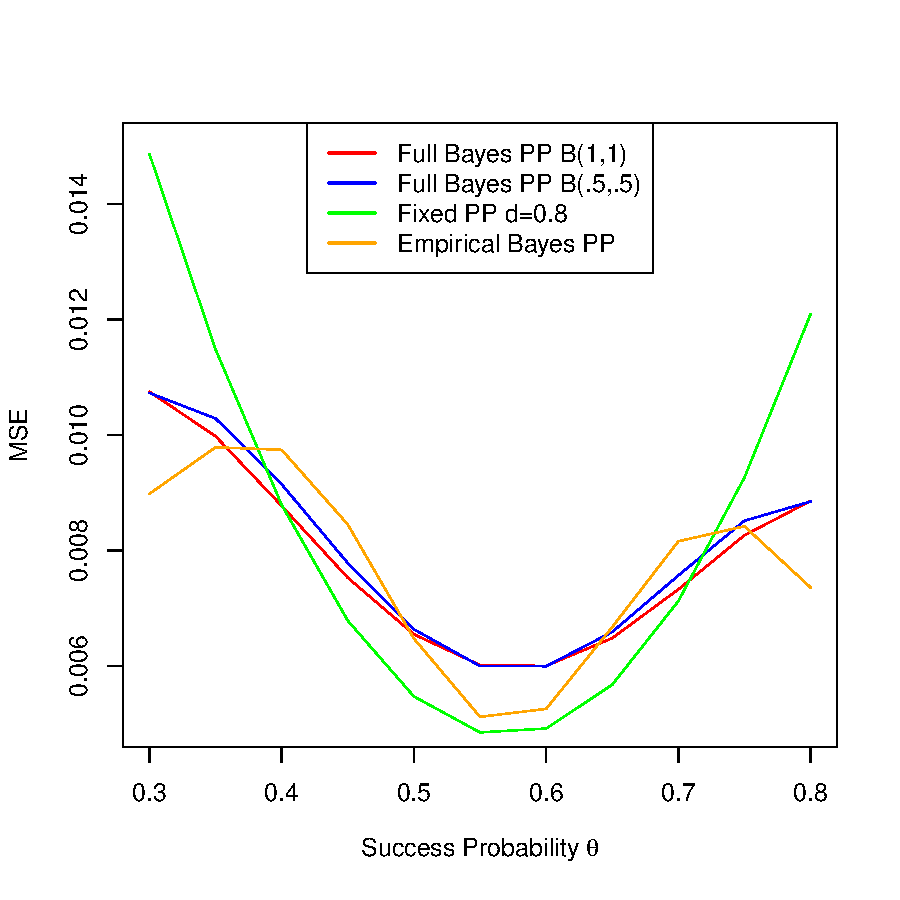
\includegraphics{Binomial-MSE}

To calculate power and type I error, we need to have a second study arm to compare against. For those functions we calculate the significance tests with sig.matrix and then calculate the operating characteristics.

\begin{Schunk}
\begin{Sinput}
> SM <- lapply(list(pp.fullbayes.11, pp.fullbayes.55, pp.fix.08, pp.eb),
+        function(PRIOR) sig.matrix(n.new, n.new, 0.95, prior=PRIOR, mc.cores = 4))
\end{Sinput}
\end{Schunk}
For power calculations we need to specify a difference between the treatment arms that we wish to detect, here 0.2.
\begin{Schunk}
\begin{Sinput}
> Difference <- 0.2
> POWER <- sapply(SM, function(SIGMAT) calc.power(sig.mat=SIGMAT, 
+       prob.rang=c(0.3,0.8), length=11, treatment.difference = Difference,
+       n.binom.control = n.new, n.binom.treatment = n.new))
> plot(p,POWER[,1],  col="red", type='l', ylab="Power",
+      xlab=expression(paste("Success Probability ",theta)))
> lines(p,POWER[,2],  col="blue")
> lines(p,POWER[,3],  col="green")
> lines(p,POWER[,4],  col="orange")
> legend("topleft", col=c("red","blue","green", "orange"), lty=1, lwd=2,
+        legend=c("Full Bayes PP B(1,1)", "Full Bayes PP B(.5,.5)",
+                 "Fixed PP d=0.8", "Empirical Bayes PP"))
\end{Sinput}
\end{Schunk}
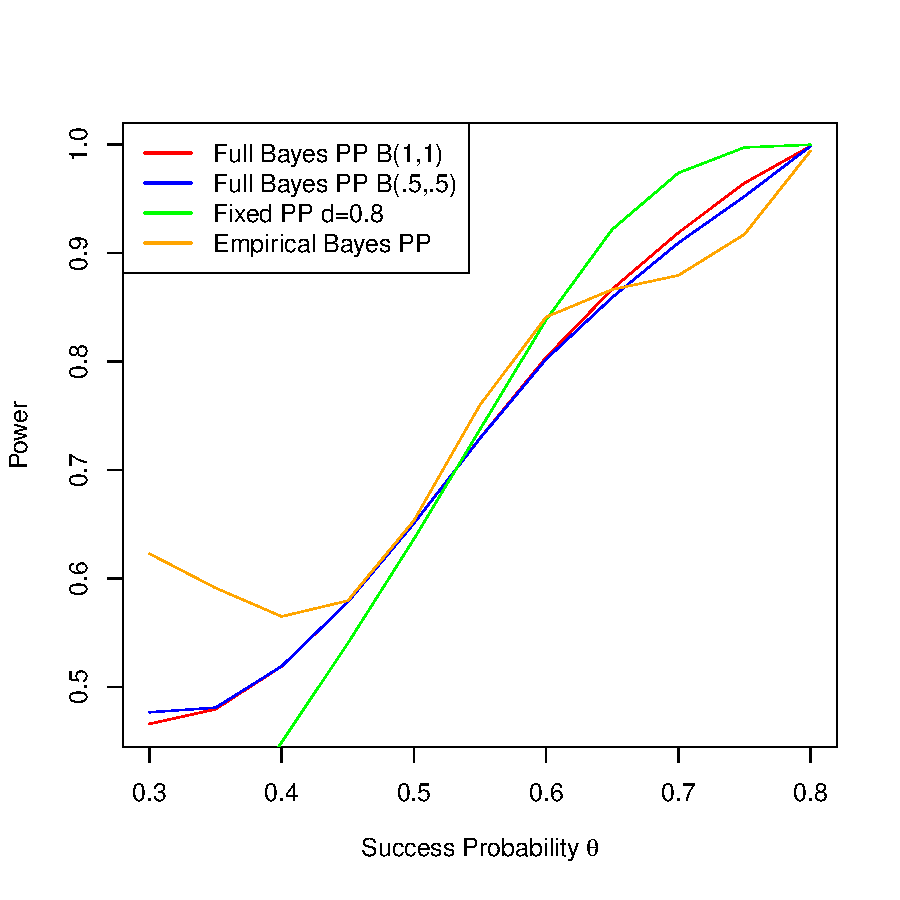
\includegraphics{Binomial-Power}


For type I error, we use the same function as for power, but we set the treatment difference to 0.
\begin{Schunk}
\begin{Sinput}
> T1E <- sapply(SM, function(SIGMAT) calc.power(sig.mat=SIGMAT, 
+          prob.rang=c(0.3,0.8), length=11, treatment.difference = 0,
+          n.binom.control = n.new, n.binom.treatment = n.new))
> plot(p,T1E[,1],  col="red", type='l', ylab="Type I Error",
+      xlab=expression(paste("Success Probability ",theta)),
+      ylim=c(0,0.15))
> lines(p,T1E[,2],  col="blue")
> lines(p,T1E[,3],  col="green")
> lines(p,T1E[,4],  col="orange")
> legend("topleft", col=c("red","blue","green", "orange"), lty=1, lwd=2,
+        legend=c("Full Bayes PP B(1,1)", "Full Bayes PP B(.5,.5)",
+                 "Fixed PP d=0.8", "Empirical Bayes PP"))
> 
\end{Sinput}
\end{Schunk}
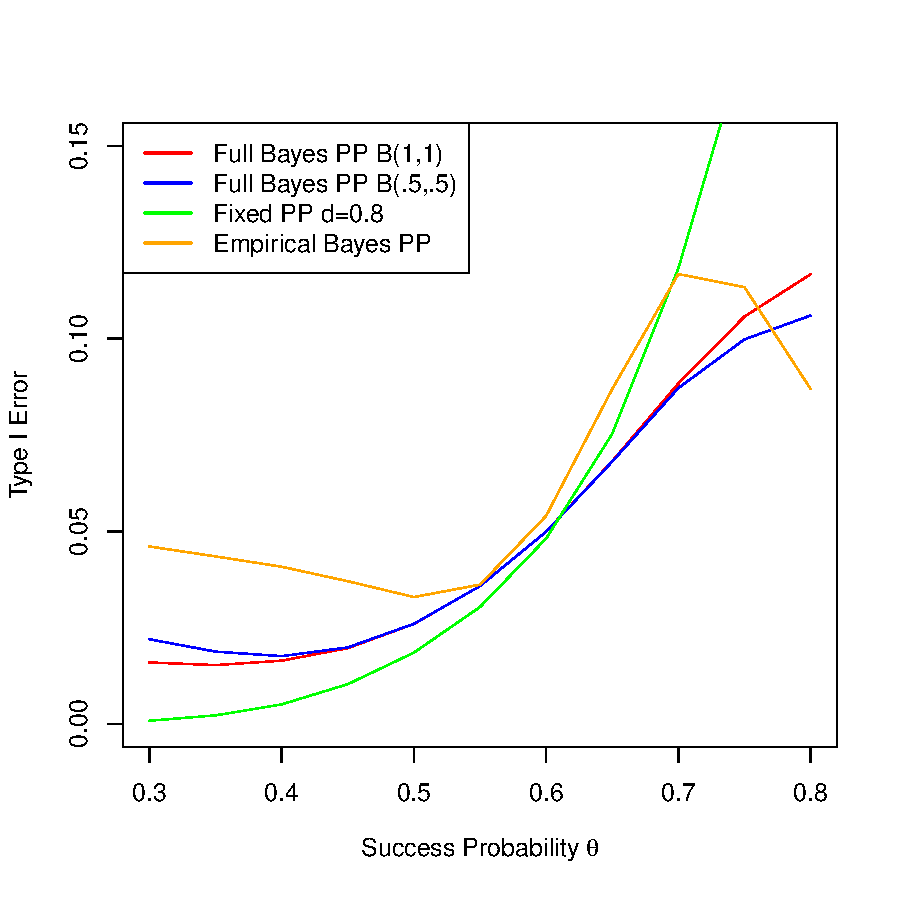
\includegraphics{Binomial-TypeIError}




\section{StudyPrior for Multiple Historical Studies}

It is also possible to use more than one historical study in the construction of the prior. Say we have 3 more studies that we want to use:

% latex table generated in R 3.3.1 by xtable 1.8-2 package
% Mon Oct 30 21:04:15 2017
\begin{table}[ht]
\centering
\begin{tabular}{rrrl}
  \hline
Study & x & n & Success \\ 
  \hline
1 & 21 & 37 & 57\% \\ 
  2 & 33 & 50 & 66\% \\ 
  3 & 23 & 40 & 57\% \\ 
  4 & 27 & 50 & 54\% \\ 
   \hline
\end{tabular}
\end{table}

With multiple historical studies, we can use the meta-analytic predictive prior of Schmidli et al. We specify the prior on the heterogeneity standard deviation in the format used by INLA. Here we use a truncated normal (which for INLA's purposes is defined on the log scale) with mean 0 and precision 1. 
\begin{Schunk}
\begin{Sinput}
> x.multi <- c(21,33,23,27)
> n.multi <- c(37,50,40,50)
> MAP <- binom.MAP.FB(x.multi, n.multi, tau.prior = list(prior= "logtnormal", param=c(0,1)))
\end{Sinput}
\end{Schunk}

The power prior can also be extended to hand multiple studies. A full Bayes approach with an independent beta prior on the weight parameters.
\begin{Schunk}
\begin{Sinput}
> PP.FB.11 <- binom.PP.FB.MC.BE(x=x.multi, n=n.multi, d.prior.a = 1, d.prior.b = 1)
> PP.FB.55 <- binom.PP.FB.MC.BE(x=x.multi, n=n.multi, d.prior.a = .5, d.prior.b = .5)
\end{Sinput}
\end{Schunk}
Or have correlation between the weight parameters, which shows good operating characteristics.
\begin{Schunk}
\begin{Sinput}
> PP.FB.COR <- binom.PP.FB.MC.COR(x=x.multi, n=n.multi, d.prior.cor = 0.5)
\end{Sinput}
\end{Schunk}
The empirical Bayes approach is also possible.
\begin{Schunk}
\begin{Sinput}
> PP.EB <- binom.PP.EB(x=x.multi, n=n.multi, X=0:n.new, N=n.new)
\end{Sinput}
\end{Schunk}


\subsection{Approximation with Mixtures}
We can approximate the priors with mixtures of densities. This makes calculations of posteriors and some operating characteristics very fast because analytical formulas are available. This is an approximation whose accuracy depends on the number of mixture components and can require some time to find all the parameters.

\begin{Schunk}
\begin{Sinput}
> MAP.approx <- conj.approx(MAP, type="beta", max.degree = 3)
> curve(MAP, n=200, lty=1, lwd=2, ylab="Density", xlab=expression(theta))
> plot(MAP.approx,  col="cyan", lwd=2, lty=2, lines.only=TRUE)
> legend("topleft", lty=1:2, col=c("black","cyan"), lwd=2, legend=c("MAP","Approximation"))
\end{Sinput}
\end{Schunk}
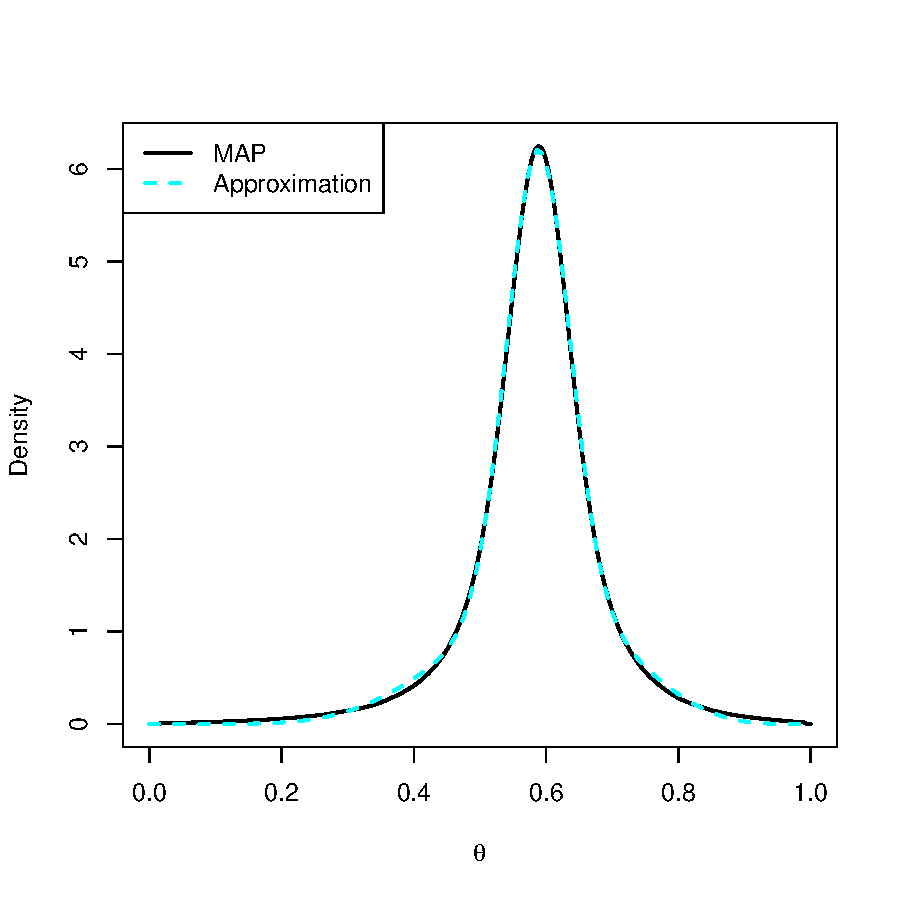
\includegraphics{Binomial-approx}
\\

Here the plot shows the original density in black and the approximation in cyan. With 3 components the approximation is very good.



\subsection{Operating Characteristics}
As before we can calculate operating characteristics. The same functions can be applied for in the single and multiple setting. Here we calculate bias and coverage.
\begin{Schunk}
\begin{Sinput}
> BIAS.PP <- sapply(list(PP.FB.11, PP.FB.55, PP.FB.COR, PP.EB), 
+                   function(PRIOR) calc.bias(PRIOR,
+                                             prob.range = c(0.3,0.8),
+                                             length=11,
+                                             n.binom=50)
+ )
\end{Sinput}
\end{Schunk}

We can also use the mixture approximations in the same functions. Note how much faster the calculations are with the approximation.
\begin{Schunk}
\begin{Sinput}
> system.time(BIAS.MAP <- calc.bias(MAP, prob.range = c(0.3,0.8),length=11,n.binom = 50))
\end{Sinput}
\begin{Soutput}
   user  system elapsed 
  4.940   0.000   4.941 
\end{Soutput}
\begin{Sinput}
> system.time(BIAS.APPROX <- calc.bias(MAP.approx, prob.range = c(0.3,0.8),length=11,n.binom = 50))
\end{Sinput}
\begin{Soutput}
   user  system elapsed 
  0.008   0.000   0.007 
\end{Soutput}
\end{Schunk}

\begin{Schunk}
\begin{Sinput}
> plot(p,BIAS.PP[,1],  col="red", type='l', ylab="Bias",
+      xlab=expression(paste("Success Probability ",theta)),
+      ylim=c(-0.15,0.15), lwd=2)
> lines(p,BIAS.PP[,2],  col="blue", lwd=2)
> lines(p,BIAS.PP[,3],  col="green", lwd=2)
> lines(p,BIAS.PP[,4],  col="orange", lwd=2)
> lines(p,BIAS.MAP,  col="black", lwd=2)
> lines(p,BIAS.APPROX,  col="cyan", lty=2, lwd=2)
> legend("topright", col=c("red","blue","green", "orange", "black","cyan"), lty=1, lwd=2,
+        legend=c("Full Bayes PP B(1,1)", "Full Bayes PP B(.5,.5)",
+                 "Full Bayes PP with Corr=.5", "Empirical Bayes PP","MAP","MAP Approx"))
> 
\end{Sinput}
\end{Schunk}
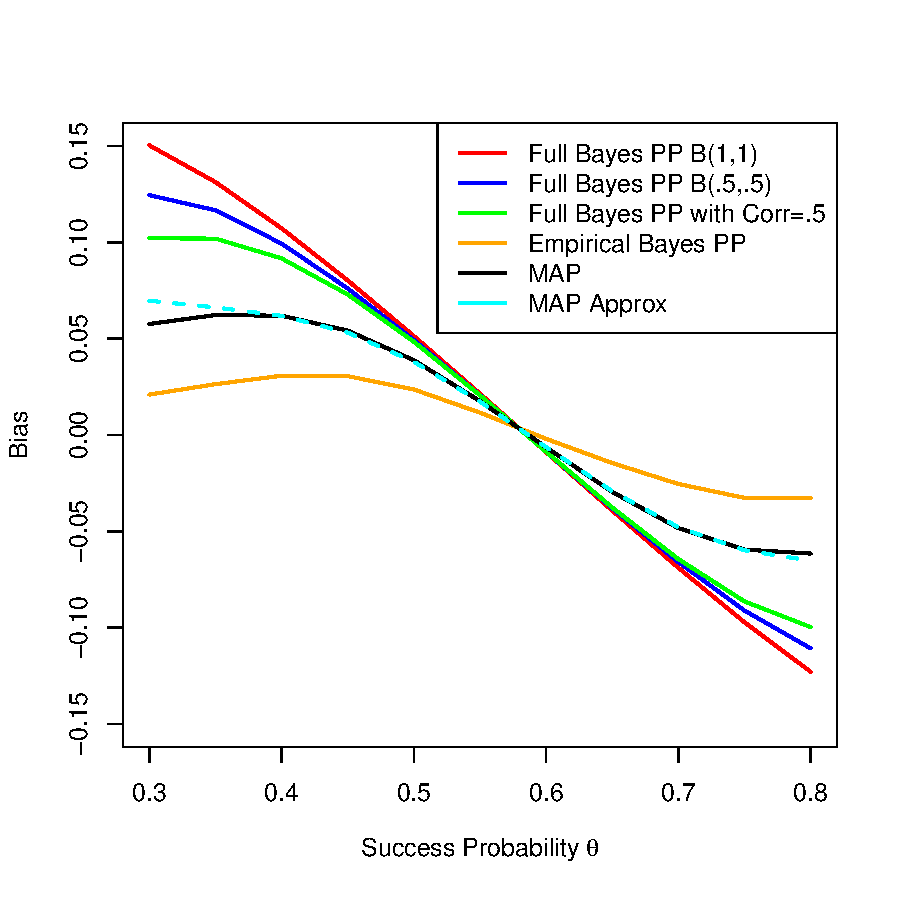
\includegraphics{Binomial-biasplot}

For calculating coverage, we implement a smoothing technique based on beta kernels. We must specify a smoothing parameter. See Bayarri for more details. 
\begin{Schunk}
\begin{Sinput}
> COVER <- sapply(list(PP.FB.11, PP.FB.55, PP.FB.COR, PP.EB, MAP), 
+                   function(PRIOR) calc.coverage(PRIOR, level = 0.95, 
+                                                 smooth = 0.05, n.control = 50))
> p2 <- seq(0.3,.8, len=501)
> plot(p2,COVER[300:800,1],  col="red", type='l', ylab="Coverage",
+      xlab=expression(paste("Success Probability ",theta)),
+      ylim=c(0,1), lwd=2)
> lines(p2,COVER[300:800,2],  col="blue", lwd=2)
> lines(p2,COVER[300:800,3],  col="green", lwd=2)
> lines(p2,COVER[300:800,4],  col="orange", lwd=2)
> lines(p2,COVER[300:800,5],  col="black", lwd=2)
> legend("bottom", col=c("red","blue","green", "orange", "black"), lty=1, lwd=2,
+        legend=c("Full Bayes PP B(1,1)", "Full Bayes PP B(.5,.5)",
+                 "Full Bayes PP with Corr=.5", "Empirical Bayes PP","MAP"))
> 
\end{Sinput}
\end{Schunk}
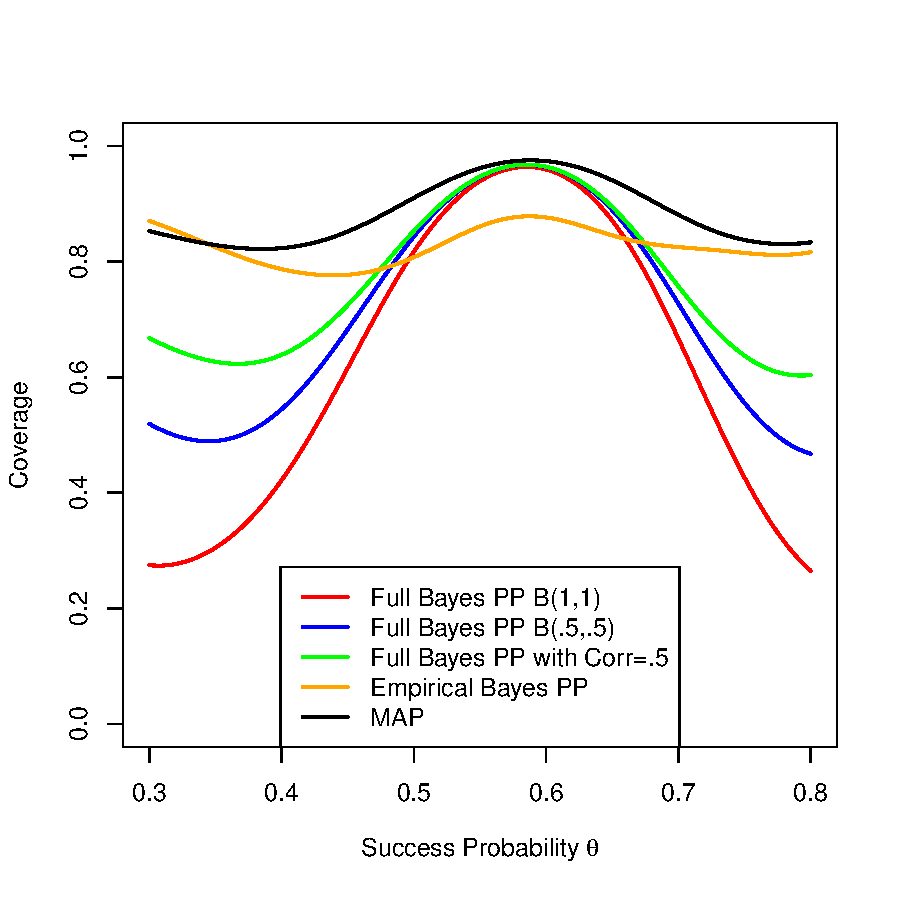
\includegraphics{Binomial-cover}


\end{document}
